% The Jordan-Wigner string (Session 5): parity factors left of site i; empty range for neighbors.
% Own drawing (Fable). Compile with: pdflatex jw_string.tex ; result moves to ../jw_string.pdf
\documentclass[11pt,tikz,border=3pt]{standalone}
\usepackage{amsmath,amssymb}
\usepackage{xcolor}
\definecolor{coursedark}{HTML}{1B2A4A}
\definecolor{courseaccent}{HTML}{7A2E8C}

\begin{document}
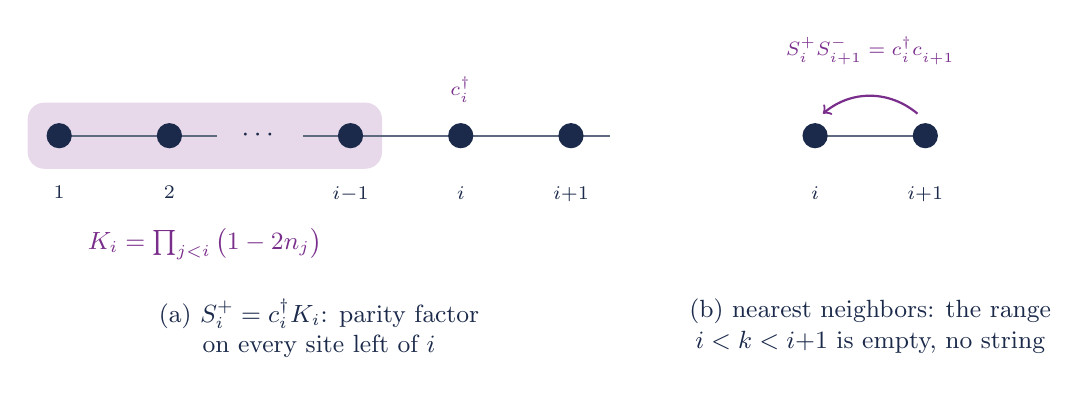
\begin{tikzpicture}[
    site/.style={circle, fill=coursedark, inner sep=0pt, minimum size=3.2mm},
    wire/.style={draw=coursedark!70, line width=0.8pt},
    lbl/.style={font=\small, text=coursedark, align=center},
    idx/.style={font=\scriptsize, text=coursedark, align=center},
  ]

  % ---- panel (a): the string K_i
  \begin{scope}[shift={(0,0)}]
    \fill[courseaccent!18, rounded corners=6pt] (-0.4,-0.42) rectangle (4.1,0.42);
    \draw[wire] (0,0) -- (2.0,0);
    \node[text=coursedark] at (2.55,0) {$\cdots$};
    \draw[wire] (3.1,0) -- (7.0,0);
    \node[site] at (0,0) {};   \node[site] at (1.4,0) {};
    \node[site] at (3.7,0) {}; \node[site] at (5.1,0) {}; \node[site] at (6.5,0) {};
    \node[idx, anchor=north] at (0,-0.52)   {$1$};
    \node[idx, anchor=north] at (1.4,-0.52) {$2$};
    \node[idx, anchor=north] at (3.7,-0.52) {$i{-}1$};
    \node[idx, anchor=north] at (5.1,-0.52) {$i$};
    \node[idx, anchor=north] at (6.5,-0.52) {$i{+}1$};
    \node[idx, text=courseaccent, anchor=south] at (5.1,0.30) {$c_i^{\dagger}$};
    \node[lbl, text=courseaccent, anchor=north] at (1.85,-1.05)
      {$K_i=\prod_{j<i}\big(1-2n_j\big)$};
    \node[lbl, anchor=north] at (3.3,-1.95)
      {(a) $S_i^{+}=c_i^{\dagger}K_i$: parity factor\\ on every site left of $i$};
  \end{scope}

  % ---- panel (b): nearest neighbors, empty string range
  \begin{scope}[shift={(9.6,0)}]
    \draw[wire] (0,0) -- (1.4,0);
    \node[site] at (0,0) {};   \node[site] at (1.4,0) {};
    \node[idx, anchor=north] at (0,-0.52)   {$i$};
    \node[idx, anchor=north] at (1.4,-0.52) {$i{+}1$};
    \draw[->, courseaccent, line width=0.8pt] (1.3,0.28) to[bend right=40] (0.1,0.28);
    \node[idx, text=courseaccent, anchor=south] at (0.7,0.78)
      {$S_i^{+}S_{i+1}^{-}=c_i^{\dagger}c_{i+1}^{\phantom{\dagger}}$};
    \node[lbl, anchor=north] at (0.7,-1.95)
      {(b) nearest neighbors: the range\\ $i<k<i{+}1$ is empty, no string};
  \end{scope}
\end{tikzpicture}
\end{document}
